\documentclass[12pt]{beamer}
\usepackage[utf8]{inputenc}
\usepackage[spanish]{babel}
\usepackage{multirow}
\usepackage{color}
\usepackage{ragged2e}
\usepackage{movie15}


\mode<presentation>{\usetheme{CambridgeUS}}
\usecolortheme{dolphin}

\title[TASMC]{Traveler Assistant System For Mexico City TASMC}
\date{}

\begin{document}

\begin{frame}
	\begin{center}
	\begin{minipage}[t]{0.8\textwidth}	
		\begin{tabular}{ccc}
			\multirow{4}{*}{
\includegraphics[height=1.7cm]{imagenes/ipn.jpg}} &
			&
     	 	\multirow{4}{*}{
\includegraphics[height=1.5cm]{imagenes/escom.jpg}} \\
      		& Instituto Politécnico Nacional & \\
      		& Escuela Superior de Cómputo & \\
      		&&\\
		\end{tabular}
	\end{minipage}
	\end{center}
	
	\begin{center}
		\small No. de Registro: 2014-A021 \\
	\end{center}		
	
	\begin{center}
		\textcolor[RGB]{0,0,204}{\Large Traveler Assistant System For Mexico City TASMC}
	\end{center}		
		
	\begin{center}
	\begin{minipage}[t]{1\textwidth}	
		\begin{tabular}{ccc}
			Presentan & 
			\multirow{4}{*}{
\includegraphics[height=1.7cm]{imagenes/logo.png}} & Directores \\
			\scriptsize Barajas Uribe Sergio & & \scriptsize  M. en C. Macario Hernández Cruz\\
			\scriptsize Vivanco Carmona Erick Rafael & & \scriptsize M. en C. Axel Ernesto Moreno Cervantes
		\end{tabular}
	\end{minipage}
	\end{center}
\end{frame}

\begin{frame}
\frametitle{Contenido}
\tableofcontents
\end{frame}

\section{Introducción}

\begin{frame}
	\frametitle{Introducción}
	\begin{block}{}
		\begin{itemize}
		\item Incremento de la transportación aérea.
		\item Creciente utilización de los dispositivos móviles.
		\item Turismo como actividad económica fundamental en México.
		\item Adaptación a los nuevos usos de los dispositivos móviles.
		\item Dispositivo móvil + Internet = Enriquece la experiencia viajera.
	\end{itemize}
	\end{block}

\end{frame}

\subsection{¿Por qué TASMC?}
\begin{frame}
	\frametitle{¿Por qué TASMC?}
	\begin{columns} 
		\begin{column}{5cm} 
			\begin{block}{Necesidades} \small 
				\begin{itemize}
					\item Precio y horario de vuelos
					\item Buscar un hotel
					\item Hacer un itinerario de viaje
				\end{itemize} 
			\end{block} 
		\end{column}
		\begin{column}{5cm} 
			\begin{center}
				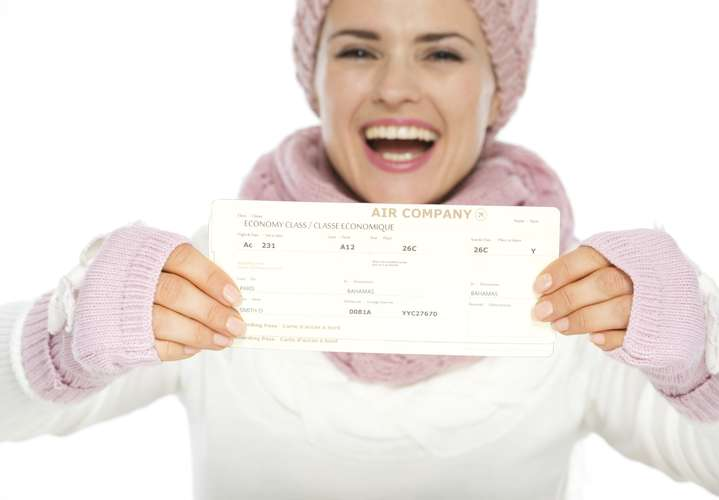
\includegraphics[height=2cm]{imagenes/nvuelo.jpg} \\
				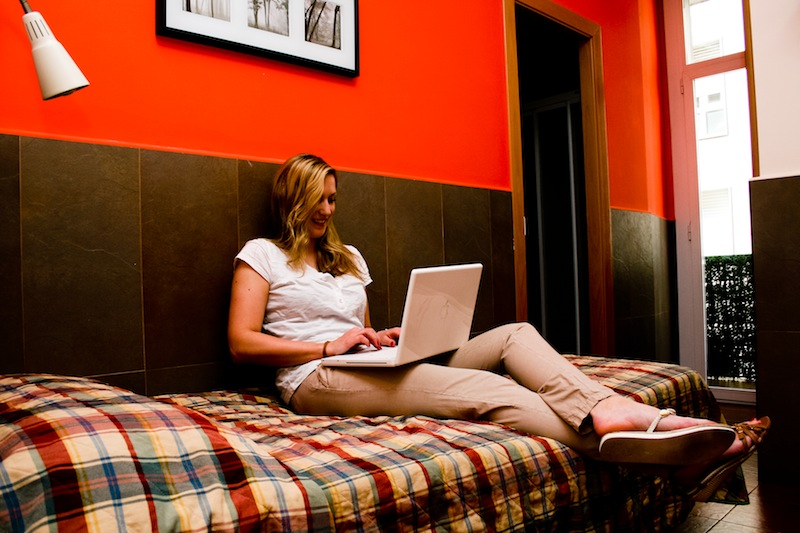
\includegraphics[height=2cm]{imagenes/nhotel.jpg} \\
				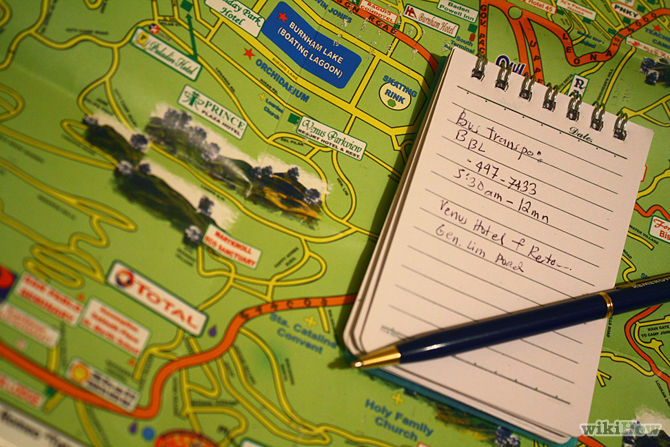
\includegraphics[height=2cm]{imagenes/nitinerario.jpg}
			\end{center} 
		\end{column} 
	\end{columns}
\end{frame}

\begin{frame}
	\frametitle{¿Por qué TASMC?}
	\begin{columns} 
		\begin{column}{5cm} 
			\begin{block}{Problemas} \small 
				\begin{itemize}
					\item Olvidar objetos 
					\item Llegar a destiempo al aeropuerto
					\item Perderse en el aeropuerto
				\end{itemize} 
			\end{block} 
		\end{column}
		\begin{column}{5cm} 
			\begin{center}
				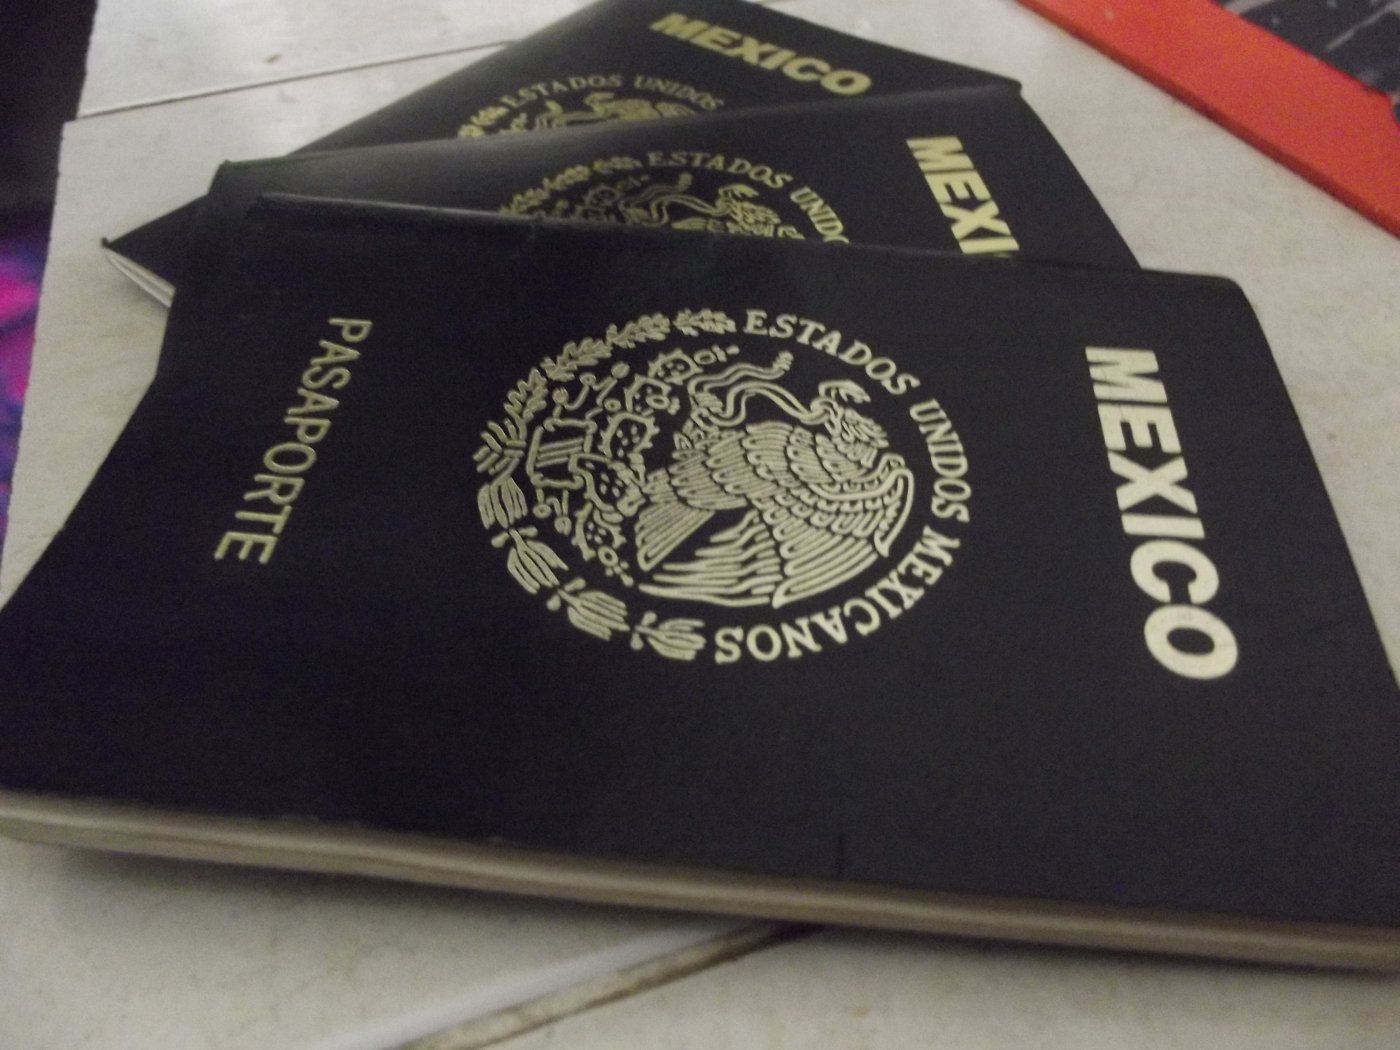
\includegraphics[height=2cm]{imagenes/pdocumento.jpg} \\
				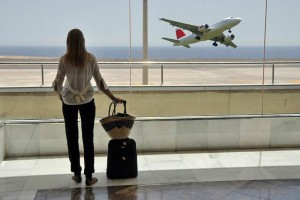
\includegraphics[height=2cm]{imagenes/pinpuntual.jpg} \\
				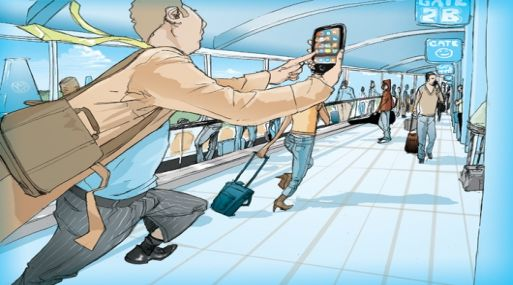
\includegraphics[height=2cm]{imagenes/pperderse.jpg}
			\end{center} 
		\end{column} 
	\end{columns}
\end{frame}

\subsection{¿Qué es TASMC?}
\begin{frame}[c]
	\frametitle{¿Qué es TASMC?}
	\begin{block}{}
		Sistema asistente para el viajero de la Ciudad de México
	\end{block}
	\begin{columns} 
		\begin{column}{5cm}
			\begin{block}{Características} \small 
				\begin{itemize}
					\item Configuración del viaje
					\item Vuelos disponibles
					\item Hoteles disponibles
					\item Lista de equipaje
					\item Itinerario de viaje
				\end{itemize} 
			\end{block} 
		\end{column}
		\begin{column}{4cm} 
			\begin{center}
				
\includegraphics[height=5cm]{imagenes/queEs.jpg}
			\end{center} 
		\end{column} 
	\end{columns}
\end{frame}

\begin{frame}[c]
	\frametitle{¿Qué es TASMC?}
	\begin{block}{}
		Sistema asistente para el viajero de la Ciudad de México
	\end{block}
	\begin{columns} 
		\begin{column}{5cm}
			\begin{block}{Características} \small 
				\begin{itemize}
					\item Ruta al aeropuerto
					\item Ubicar dentro del AICM
					\item Información del vuelo
					\item Ruta del vuelo
				\end{itemize} 
			\end{block} 
		\end{column}
		\begin{column}{4cm} 
			\begin{center}
				
\includegraphics[height=5cm]{imagenes/queEs.jpg}
			\end{center} 
		\end{column} 
	\end{columns}
\end{frame}

\subsection{Objetivo de TASMC}

\begin{frame}
	\frametitle{Objetivo de TASMC}
	\begin{block}{}
		\justifying
		Diseñar un sistema integral de gestión para las actividades del viajero del AICM, al brindarle la información 						necesaria en su dispositivo móvil para hacer posible la organización integral del viaje e incentivar la demanda 					potencial de servicios de transportación aérea de viajes turísticos o de negocios en México.
	\end{block}
\end{frame}

\subsection{Mobile-D}

\begin{frame}
	\frametitle{Mobile-D}
	\begin{block}{Objetivo}
		Conseguir ciclos de desarrollo muy rápidos en equipos muy pequeños trabajando en un mismo espacio físico.
	\end{block}
	\begin{block} \small 
		\begin{itemize}
			\item 	Programación Extrema (XP)
			\item Crystal Methodologies
			\item Proceso Unificado de Desarrollo (RUP)
		\end{itemize} 
	\end{block}
\end{frame}

\begin{frame}
	\frametitle{Ciclo de Desarrollo Mobile-D}
	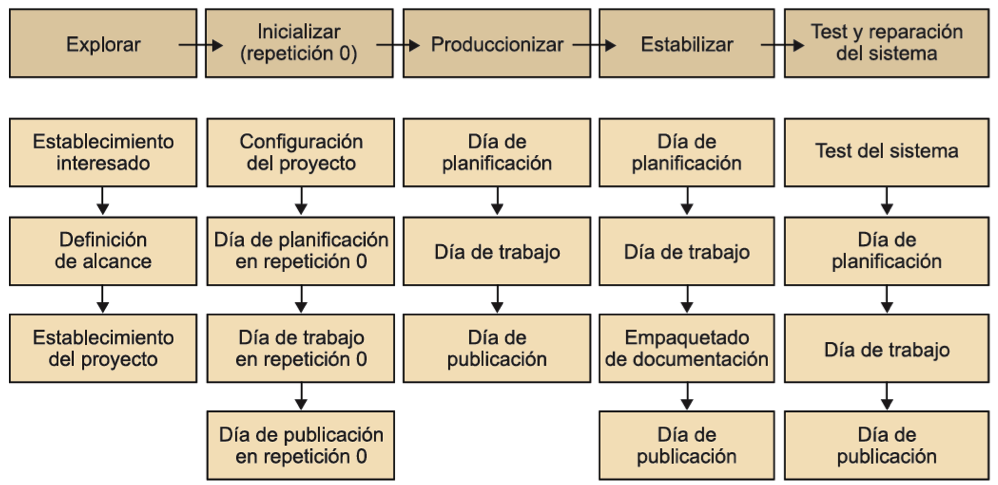
\includegraphics[height=5cm]{imagenes/mobiled.png}
\end{frame}

\section{Análisis y Diseño}

\begin{frame}
	\frametitle{Hardware}
	\begin{block}{	Equipos de cómputo para:}
	\begin{itemize}
		\item Desarrollo de la aplicación móvil.
		\item La aplicación web de administración y servicio web.
	\end{itemize}
	\end{block}
	
	\begin{block}{	Teléfono inteligente con:}
	\begin{itemize}
		\item Magnetómetro (brújula)
		\item Acelerómetro
		\item Giroscopio
	\end{itemize}
	\end{block}
\end{frame}

\begin{frame}
	\frametitle{Hardware}
	\begin{columns} 
		\begin{column}{2cm}
			\begin{center}
				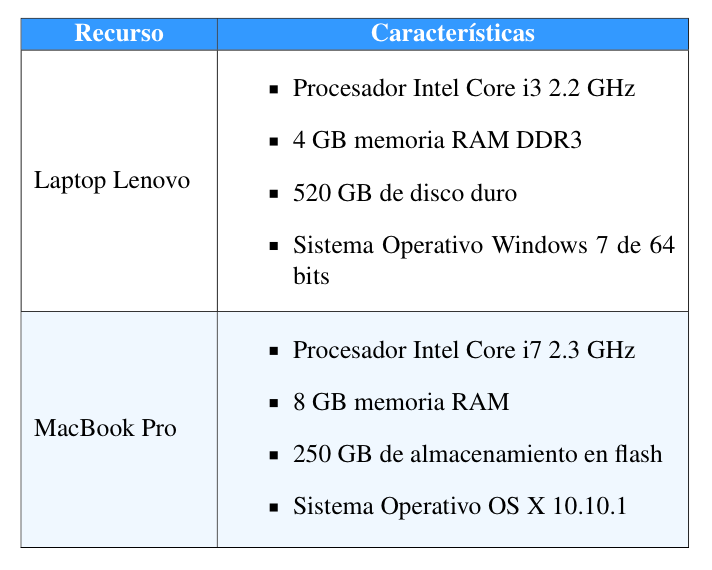
\includegraphics[height=3cm]{imagenes/computadoras.png}
			\end{center}
		\end{column}
		\begin{column}{5cm} 
			\begin{center}
				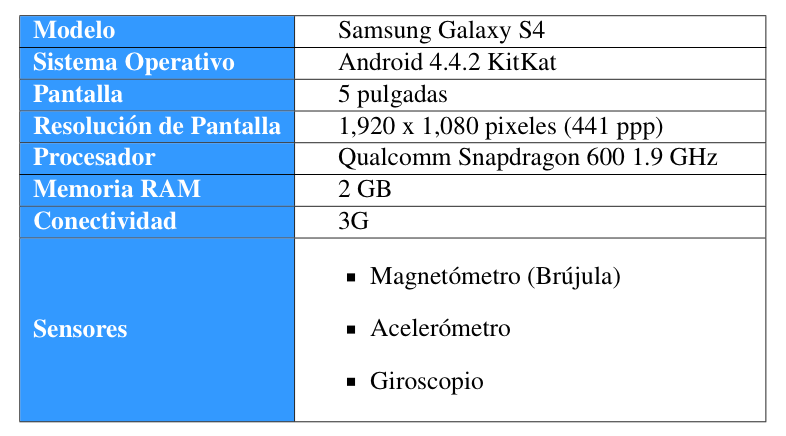
\includegraphics[height=3cm]{imagenes/telefono.png}
			\end{center} 
		\end{column} 
	\end{columns}
\end{frame}


\begin{frame}
	\frametitle{Software}
		El software que se necesita consta de: 
		\begin{itemize}
		 	\item Sistemas operativos (Windows, Mac OS y Android)
		 	\item IDE (Android Studio)
		 	\item Herramienta UML (StarUML)
		 	\item SGBD (MySQL y SQLite)
		 	\item Servidor (Apache)
		 	\item APIs (Google maps, IndoorAtlas)
		 	\item Lenguajes de Programación (Java y PHP)		 	
		\end{itemize}
\end{frame}


\begin{frame}
	\frametitle{Factibilidad Económica}
	\begin{columns} 
		\begin{column}{5cm}
			\begin{block}{Recursos Humanos}
				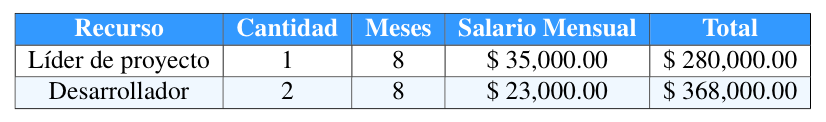
\includegraphics[height=0.8cm]{imagenes/rh.png}
			\end{block}
			\begin{block}{Recursos Consumibles}
				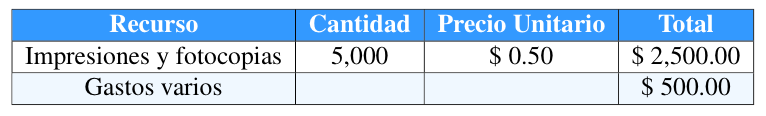
\includegraphics[height=1cm]{imagenes/rc.png}
			\end{block}
		\end{column}
		\begin{column}{5cm} 
			\begin{block}{Recursos Tecnológicos}
				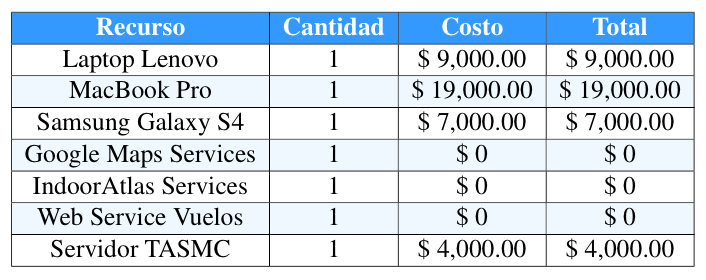
\includegraphics[height=2cm]{imagenes/rt.png}
			\end{block}
			\begin{block}{Costo Total TASMC}
				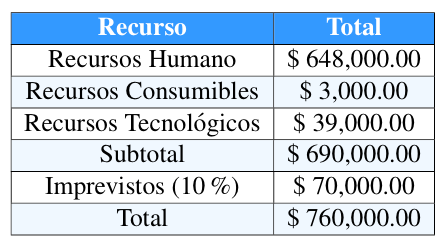
\includegraphics[height=2.5cm]{imagenes/ct.png}
			\end{block}
		\end{column} 
	\end{columns}
\end{frame}


\begin{frame}
		\frametitle{Factibilidad Operativa}
		\begin{block}{Recursos humanos}
			\begin{itemize}
			\item Equipo de trabajo con conocimientos necesarios.
			\item Experiencia en desarrollo.
			\end{itemize}
		\end{block}
		\begin{block}{Recursos necesarios}
			\begin{itemize}
			\item Proyecto como prototipo.
			\item Extensión y mejora
			\end{itemize}
		\end{block}
\end{frame}


\begin{frame}
	\frametitle{Reglas de Negocio}
	\begin{block}{RN de tipo Hecho}
	\begin{center}
	

	\begin{tabular}{c|l}
			RN05 & Visualizar los vuelos de las aerolíneas \\
			RN07 & Notificar al viajero \\
			RN08 & Recordar documentos importantes\\
      		RN09 & Puntualidad en el aeropuerto\\
      		RN10 & Guardar objetos importantes\\
      		RN11 & Hoteles en la ciudad destino\\
      		RN12 & Usabilidad\\
      		RN13 & Disponibilidad\\
      		RN14 & Información del AICM\\
		\end{tabular}
			\end{center}
		\end{block}
\end{frame}


\begin{frame}
	\frametitle{Requerimientos Funcionales}
	\begin{block}{}
	\begin{center}
	

	\begin{tabular}{c|l}
			RF01 & Configurar gustos y posibilidades económicas \\
			RF02 & Visualizar sugerencias de hoteles \\
			RF03 & Visualizar sugerencias de vuelos\\
      		RF04 & Mostrar lista de objetos\\
      		RF05 & Permitir generar un itinerario de viaje\\
      		RF06 & Mostrar una ruta para llegar al AICM\\
      		RF07 & Ubicar al usuario dentro del AICM\\
      		RF08 & Mostrar la información del vuelo\\
		\end{tabular}
			\end{center}
		\end{block}
\end{frame}


\begin{frame}
	\frametitle{Requerimientos No Funcionales}
	\begin{block}{}
	\begin{center}
	

	\begin{tabular}{c|l}
			RNF01 & El entorno no debe afectar la localización.\\
			RNF02 & Disponible para Android 4.4\\
			RNF03 & Interfaz gráfica acorde al funcionamiento del sistema.\\
      		RNF04 & Velocidad del sistema acorde a la disponibilidad de la red.\\
      		RNF05 & Escalibilidad.\\
      		RNF06 & Soporte contínuo al sistema\\
      		RNF07 & Navegación de fácil entendimiento y de manera intuitiva.\\
		\end{tabular}
			\end{center}
		\end{block}
\end{frame}


\begin{frame}
	\frametitle{Arquitectura TASMC}
	\begin{center}
		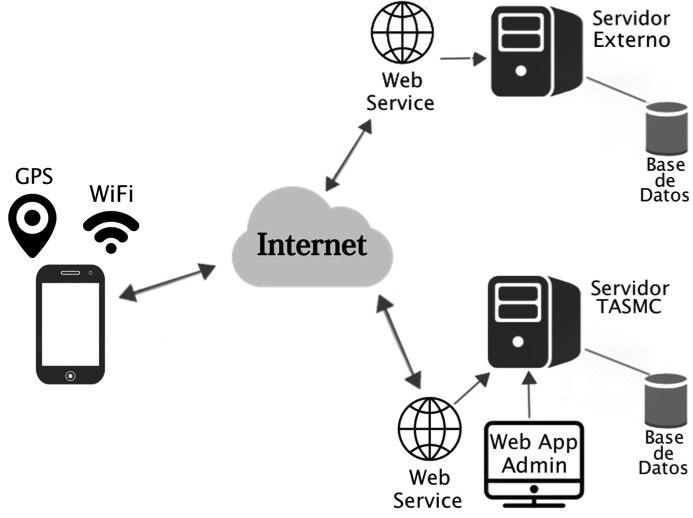
\includegraphics[height=6.5cm]{imagenes/arquitectura.png}	
	\end{center}
\end{frame}


\begin{frame}
	\frametitle{Diagrama de casos uso general del Administrador}
	\begin{center}
		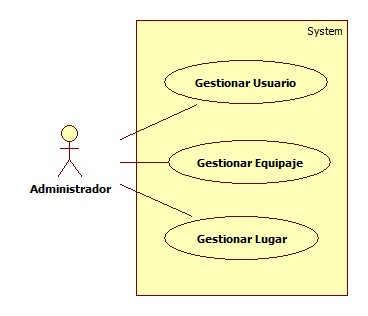
\includegraphics[height=6.5cm]{imagenes/cugeneralAdministrador.jpg}	
	\end{center}
\end{frame}


\begin{frame}
	\frametitle{Diagrama de casos uso general del Usuario}
	\begin{center}
		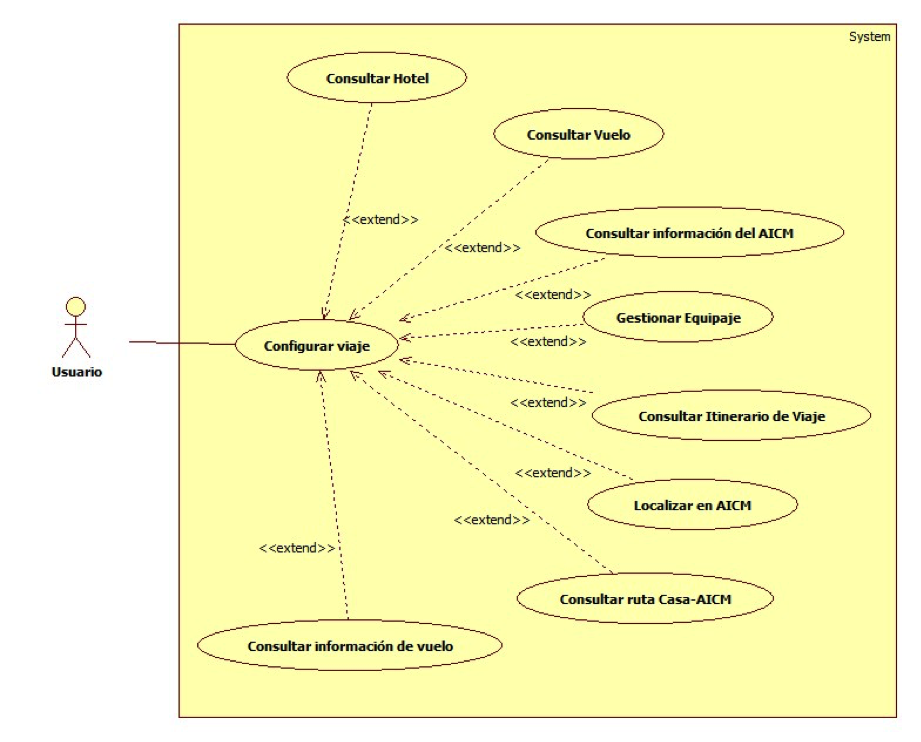
\includegraphics[height=6.5cm]{imagenes/cugeneralUsuario.png}	
	\end{center}
\end{frame}


\begin{frame}
	\frametitle{Diagrama de clases}
	\begin{center}
		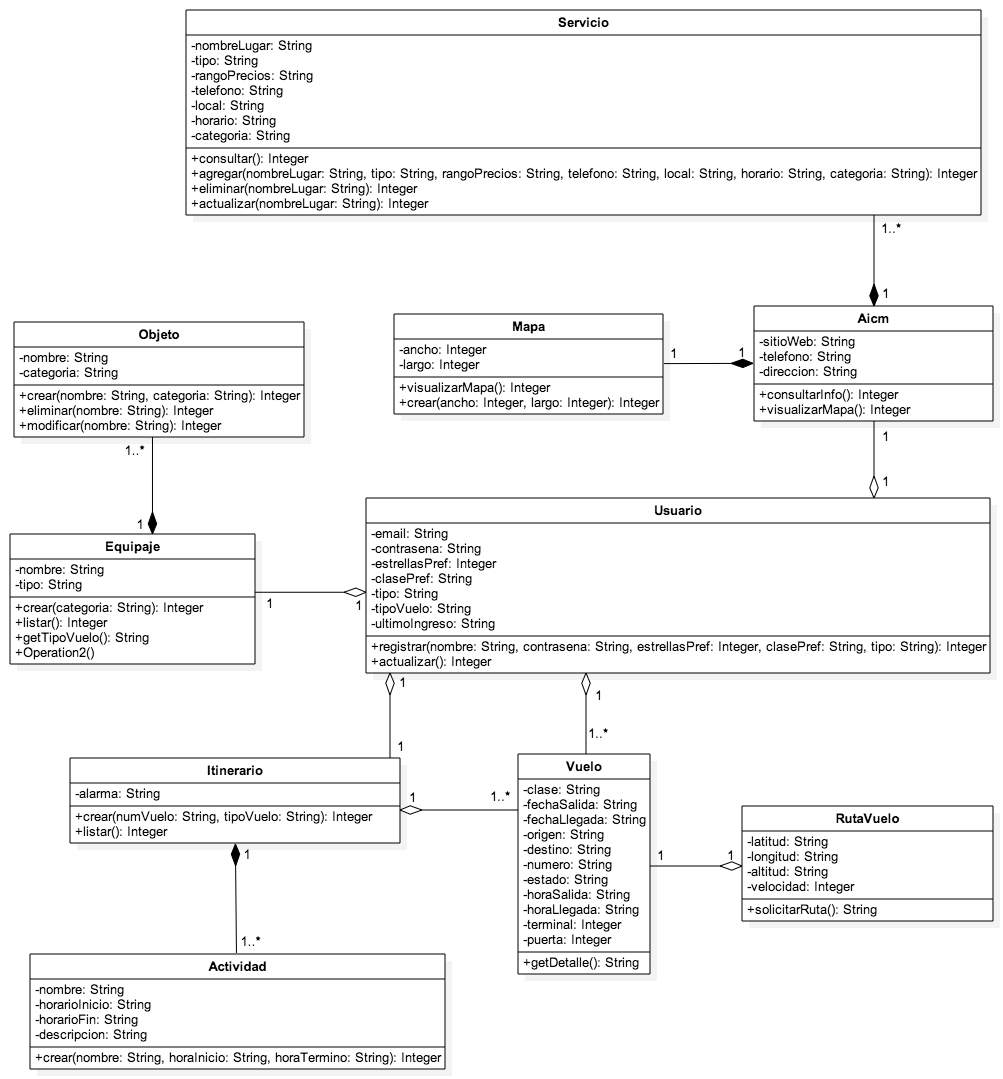
\includegraphics[height=6.5cm]{imagenes/diagramaClasesMovil.png}	
	\end{center}
\end{frame}


\begin{frame}
	\frametitle{Diagrama de secuencia Consultar Vuelo}
	\begin{center}
		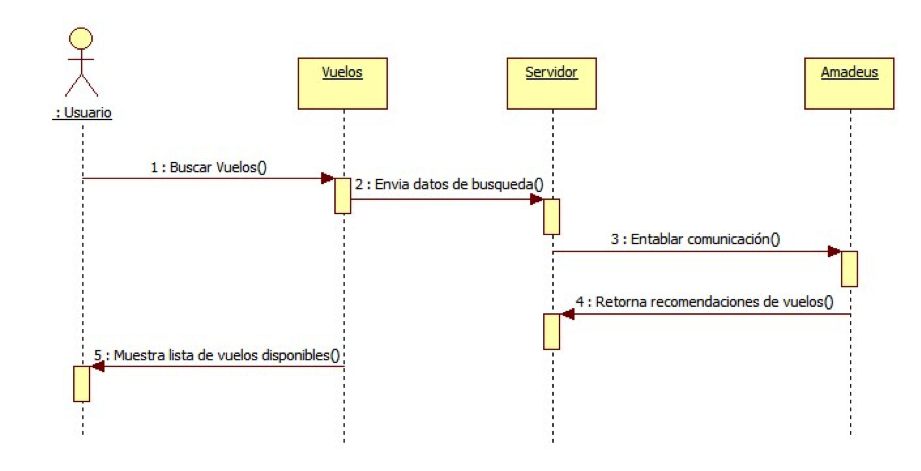
\includegraphics[height=6.5cm]{imagenes/secConsultarVuelo.png}	
	\end{center}
\end{frame}

\begin{frame}
	\frametitle{Diagrama de secuencia Gestionar Equipaje}
	\begin{center}
		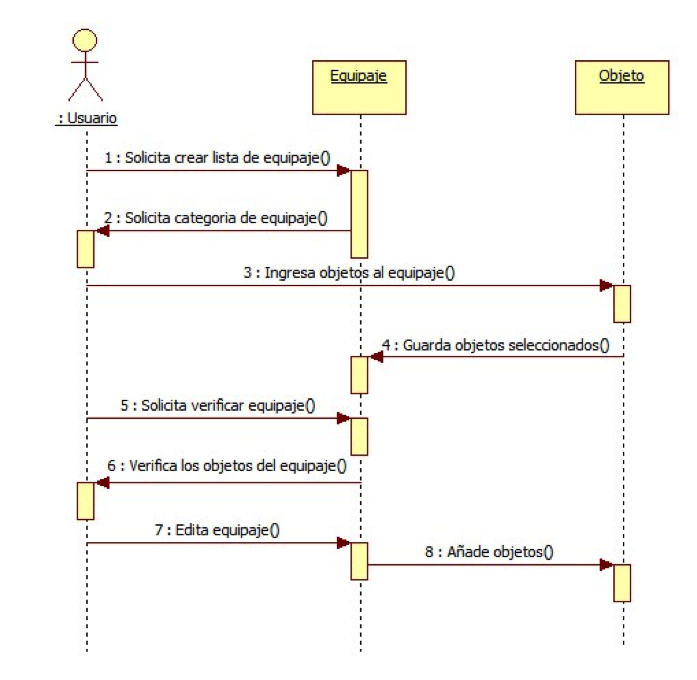
\includegraphics[height=7cm]{imagenes/secGestionarEquipaje.png}	
	\end{center}
\end{frame}

\begin{frame}
	\frametitle{Diagrama de secuencia Gestionar Lugar}
	\begin{center}
		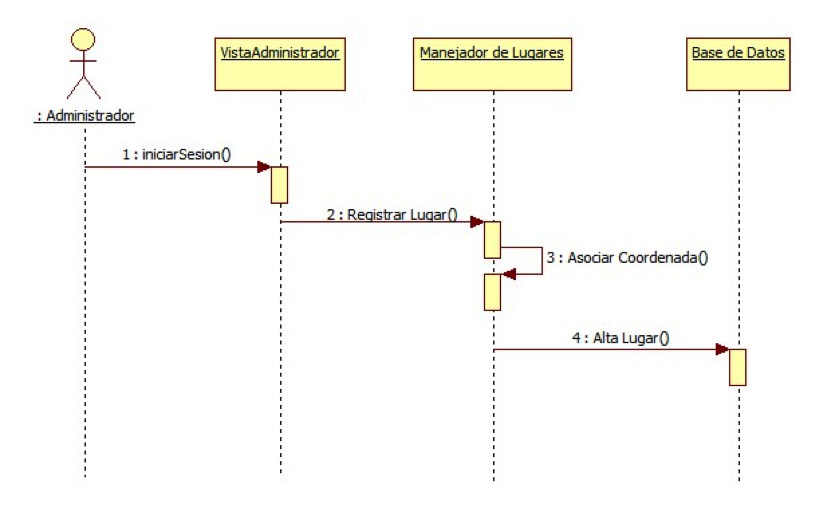
\includegraphics[height=6.5cm]{imagenes/secGestionarLugar.png}	
	\end{center}
\end{frame}

\begin{frame}
	\frametitle{Interfaz Gráfica}
	\begin{block}{}
	\includemovie[
  		poster,
  		text=(ejemplo),
  		autorun,
  		repeat]{.5\linewidth}{.375\linewidth}{video.mov}
   \end{block}
\end{frame}

\section{Trabajo Futuro}

\begin{frame}
	\frametitle{Trabajo a Futuro}
	\begin{block}{}
		\begin{itemize}
	\item Producción
	\item Estabilización
	\item Pruebas
\end{itemize}
	\end{block}

\end{frame}  

\begin{frame}
	\begin{center}
		\Large ¡Gracias por su atención!
	\end{center}
\end{frame}

\end{document}